\documentclass[12pt]{article}
\usepackage{xr-hyper}
\externaldocument{/Users/shenyan3/Documents/full_house_model/supplement}
\usepackage{hyperref}
\usepackage[english]{babel}
\usepackage{graphicx}
\usepackage{framed}
\usepackage[normalem]{ulem}
\usepackage{amsmath}
\usepackage{amsthm}
\usepackage{amssymb}
\usepackage{amsfonts}
\usepackage{enumerate}
\usepackage{graphicx} % Allows including image
\usepackage{mathtools}
\hypersetup{
  linkcolor  = blue,
  citecolor  = blue,
  urlcolor   = blue,
  colorlinks = true,
} % color setup
\usepackage[utf8]{inputenc}
\usepackage[margin=1in]{geometry}
\usepackage{float} % for "H" placement specifier
\usepackage[authoryear]{natbib}
\usepackage{indentfirst}
\usepackage[dvipsnames]{xcolor}
\usepackage{array}
\usepackage{subcaption}
\usepackage{caption}
\usepackage[T1]{fontenc}
\usepackage{tikz}
\newcommand{\fatterdot}{\raisebox{0.15ex}{\tikz\filldraw[black,x=1.5pt,y=1.5pt] (0,0) circle (1);}}
\newcommand{\xn}{x^{\frac{1}{n}}}
\newcommand{\xnone}{x^{\frac{1}{n+1}}}

\newcommand{\R}{\mathbb{R}}
\DeclareUnicodeCharacter{FB01}{fi}
\DeclareUnicodeCharacter{FF0C}{,}
\DeclareMathOperator*{\Prob}{P}
\DeclareMathOperator*{\argmax}{arg\,max}
\DeclareMathOperator*{\argmin}{arg\,min}
\setlength\extrarowheight{1pt}

\newcommand\red[1]{{\color{red}#1}}

\bibliographystyle{plainnat}

\newtheorem{theorem}{Theorem}[section]
\newtheorem{corollary}{Corollary}[theorem]
\newtheorem{lemma}[theorem]{Lemma}
\newtheorem{prop}[theorem]{Proposition}
\newtheorem{defn}[theorem]{Definition}
\allowdisplaybreaks

\title{Additional Batting Average Reults}
\author{Daniel J. Eck$^1$, Shen Yan$^1$\thanks{Daniel J. Eck (\url{dje13@illinois.edu}); email addresses: Shen Yan (\url{shenyan3@illinois.edu})}}

\date{}

\begin{document}

\maketitle

{\centering
1. Department of Statistics, University of Illinois Urbana-Champaign \\}



\section{Supplement}

Get main text \\

We now apply Theorem~\ref{theorem:normalgeneral} and the reliability guarantees in Theorem~\ref{theorem:asymptotic} to evaluate the contextual extremeness of observed outcomes in a real-world system where the underlying distribution of aptitude is not directly observable and evolves over time. Major League Baseball (MLB) offers a canonical example of such a system. Here, player skill (latent batting aptitude) is inferred only indirectly through season-level observed outcomes (batting averages), which are shaped by changing population structures and environmental variance. See Figure~\ref{Fig:means-sd-full-time} presents smoothed estimates of the mean and standard deviation of batting averages for full-time players from 1871 to 2023.
\begin{figure}[t!]
\begin{center}
	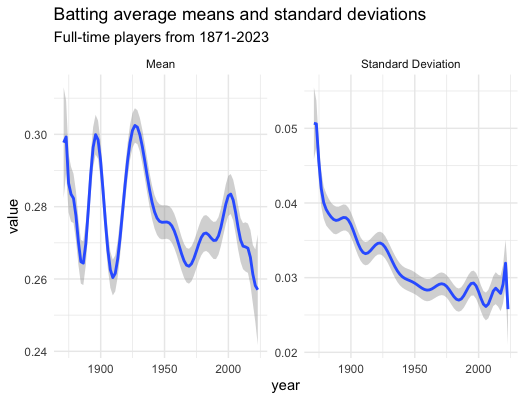
\includegraphics[scale=0.75]{means-sd-full-time.png}
\end{center}
\caption{Seasonal means and standard deviations of batting averages for full-time players from 1871-2023. Smoothing is applied to both trends.}
\label{Fig:means-sd-full-time}
\end{figure}

In particular, MLB introduced a series of rule changes in 2023 intended to increase in-game action, including a restriction on defensive positioning designed to raise batting averages on balls in play (BABIP) \citep{castrovince2023mlb}. 

First, the 2023 mean batting average for full-time players increased by 0.0057 (corresponding to an additional hit about every four baseball games) with a reduction in variability. A two-sample tests for differences in batting averages among full-time players from the 2023 and 2022 seasons has a p-value of 0.039. Thus, the rule changes seemed to be effective in yielding increased batting averages\footnote{Technically, \cite{castrovince2023mlb} referred to MLB's desire to increased batting averages on balls in play (BABIP) while this analysis focused on batting averages. BABIP increased by 0.0061 from 2022 to 2023.} Moreover, the 2023 MLB batting leader Luis Arraez had a 0.354 batting average which was the first batting average to exceed .350, a mark of excellence, since Josh Hamilton in 2010. 

Now we turn to applying the results of Theorem~\ref{theorem:normalgeneral} in this example to contextualize the effect of these rule changes. Here we assume that seasonal batting averages of full-time players are normally distributed. The true means and standard deviations of these distributions are unknown. Thus, we estimate them via plug-in sample mean and sample standard-deviation and invoke the reliability guarantees from Theorem~\ref{theorem:asymptotic}. Notably, we see from Figure~\ref{Fig:means-sd-full-time} that both the average and variability of batting averages in 2023 are among the lowest observed in the dataset, indicating a historically suppressed environment for batting averages of full-time batters.

\begin{figure}[t!]
\begin{center}
	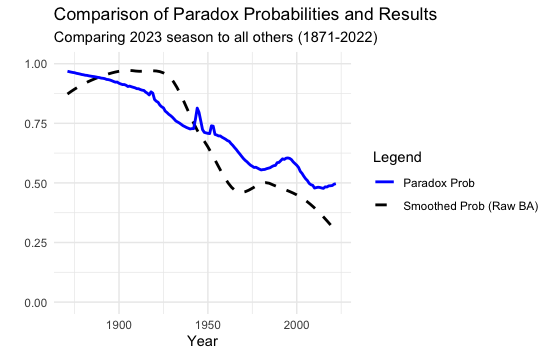
\includegraphics[scale=0.75]{paradox-prob-results.png}
\end{center}
\caption{Comparison of paradox probabilities and empirical exceedance rates relative to the 2023 season, based on data from 1871-2022. The blue line shows estimated paradox probabilities via plug-in using Theorem~\ref{theorem:normalgeneral}. The black dashed line displays a smoothed empirical exceedance rate for Arraez's 2023 batting average.}
\label{Fig:paradox-prob-results}
\end{figure}

We now apply Theorem~\ref{theorem:normalgeneral} to quantify paradox probabilities for extreme batting averages when comparing the 2023 season to all prior seasons. We treat the 2023 season as system~1 and each season from 1871 to 2022 as system~2. Figure~\ref{Fig:paradox-prob-results} displays the resulting paradox probabilities \eqref{eq:paradoxnormal}, estimated via plug-in using sample means and standard deviations. Because these estimators are $\sqrt{n}$-consistent, the reliability guarantees of Theorem~\ref{theorem:asymptotic} apply.

For comparison, Figure~\ref{Fig:paradox-prob-results} also reports a smoothed empirical exceedance rate, defined as the proportion of historical seasons in which the maximum batting average exceeded Luis Arraez's 2023 mark. The estimated paradox probabilities closely track this empirical benchmark. Both quantities increase steadily as one moves backward in time, reflecting the fact that earlier eras---characterized by higher means, larger variances, and smaller effective populations---were structurally more conducive to producing extreme observed batting averages, even if underlying talent levels were lower.

Under Full House Modeling, Arraez's 2023 performance ranks 68th all-time among full-time batters after accounting for population depth and contextual effects \citep{yan2025comparing, fullhouse2025}, in contrast to his raw observed rank of 341. This discrepancy illustrates how observed dominance can be distorted by changes in population structure and measurement environments. Paradox probabilities provide a formal way to quantify this distortion, clarifying why exceptional modern performances may appear historically unremarkable when evaluated without contextual adjustment.


\begin{figure}[ht!]
\begin{center}
	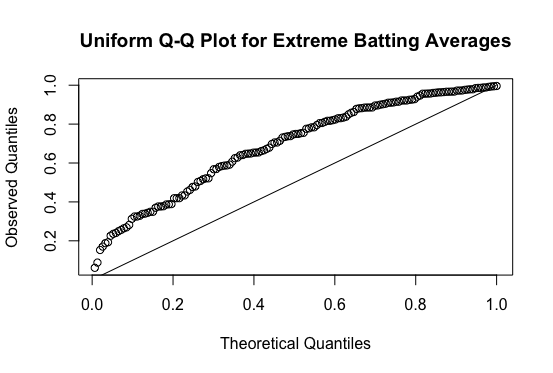
\includegraphics[scale=0.75]{uniform-qq.png}
\end{center}
\caption{Uniform Q-Q plot for extreme batting averages defined as $\widehat{F}(Y_{(n_i),i})^{n_i}$ where $i$ denotes the season, $n_i$ denotes the number of full-time players in season $i$, $Y_{(n_i),i}$ denotes the highest batting average for full-time players in season $i$, and $\widehat{F}$  is the distribution function of the normal distribution with sample mean and standard deviation estimators substituted for the population parameters.}
\label{Fig:uniform-qq}
\end{figure}

\cite{yan2025comparing} studied historical batting averages and era-adjusted batting averages through Full House Modeling for Luis Arraez's 2023 seasons and Jeff McNeil's MLB leading 2022 season in which he hit 0.326. They found that when one accounts for park and era effects then Arraez and McNeil had very similar performances, despite Arraez's large lead in raw batting average. These authors also found that assuming normality for batting averages among full-time players might not be appropriate \citep{yan2025fullhouse-supplement}. Even so, we evaluate $\widehat{F}(Y_{(n_i),i})^{n_i}$, the observed percentile of the distribution for the maximum batting average $Y_{(n_i),i}$ in season $i$. These percentiles are not uniformly distributed as seen in Figure~\ref{Fig:uniform-qq}. 

Interestingly, the percentile corresponding to Luis Arraez's 2023 MLB leading batting average is largely without recent precedent. See Table~\ref{Tab:extreme-performers} for specifics. This table contains information from all seasons in which an MLB leading batter's extreme batting average percentile exceeds that of Luis Arraez in 2023. Notice that there is a significant drop off in the frequency of such seasons after Rogers Hornsby's modern day (post-1900) record 0.424 season from 1924. It is also interesting to note that the four most recent seasons in this table are from international players or players that would not have been allowed to play baseball had segregation continued (same with Rod Carew in 1977). Again, extreme performances were more common when the talent pool was more restricted and batting strategies and training methods were more variable, not when MLB expanded the number of teams \citep{Gould96, DE20, DE20b, yan2025fullhouse-supplement}. This table also includes a column for p-values from a Shapiro-Wilk test \citep{shapiro1965analysis} on the normality of batting average for full-time players. These results support the findings in \cite{yan2025fullhouse-supplement}. Moreover, the values $\widehat{F}(Y_{(n_i),i})^{n_i}$ do not follow a uniform distribution as indicated in Figure~\ref{Fig:uniform-qq}.
 
\begin{table}[H]
\centering
\begin{tabular}{rlcccc}
  \hline
Year & Name & MLB leading BA & n & Shapiro Wilk p-value & Extreme Percentile \\ 
  \hline
1876 & Ross Barnes & 0.429 & 40 & 0.0043 & 0.9791 \\ 
  1881 & Cap Anson & 0.399 & 42 & 0.3213 & 0.9665 \\ 
  1884 & Fred Dunlap & 0.412 & 110 & 0.0066 & 0.9722 \\ 
  1887 & Tip O'Neill & 0.435 & 112 & 0.0352 & 0.9848 \\ 
  1901 & Nap Lajoie & 0.426 & 104 & 0.3360 & 0.9760 \\ 
  1904 & Nap Lajoie & 0.376 & 104 & 0.0402 & 0.9861 \\ 
  1905 & Cy Seymour & 0.377 & 112 & 0.0437 & 0.9602 \\ 
  1908 & Honus Wagner & 0.354 & 115 & 0.0462 & 0.9614 \\ 
  1909 & Ty Cobb & 0.377 & 111 & 0.0937 & 0.9673 \\ 
  1910 & Nap Lajoie & 0.383 & 118 & 0.0082 & 0.9775 \\ 
  1911 & Ty Cobb & 0.420 & 115 & 0.0416 & 0.9663 \\ 
  1912 & Ty Cobb & 0.409 & 126 & 0.0001 & 0.9730 \\ 
  1913 & Ty Cobb & 0.390 & 119 & 0.0132 & 0.9570 \\ 
  1916 & Tris Speaker & 0.386 & 114 & 0.0003 & 0.9915 \\ 
  1917 & Ty Cobb & 0.383 & 117 & 0.0890 & 0.9724 \\ 
  1918 & Ty Cobb & 0.382 & 109 & 0.4605 & 0.9575 \\ 
  1922 & George Sisler & 0.420 & 118 & 0.0174 & 0.9671 \\ 
  1924 & Rogers Hornsby & 0.424 & 118 & 0.1749 & 0.9863 \\ 
  1941 & Ted Williams & 0.406 & 110 & 0.0104 & 0.9946 \\ 
  1957 & Ted Williams & 0.388 & 117 & 0.0534 & 0.9885 \\ 
  1977 & Rod Carew & 0.388 & 196 & 0.2965 & 0.9935 \\ 
  1980 & George Brett & 0.390 & 184 & 0.0400 & 0.9960 \\ 
  1985 & Wade Boggs & 0.368 & 190 & 0.0417 & 0.9885 \\ 
  1988 & Wade Boggs & 0.366 & 180 & 0.0573 & 0.9789 \\ 
  1994 & Tony Gwynn & 0.394 & 153 & 0.0392 & 0.9631 \\ 
  2002 & Barry Bonds & 0.370 & 209 & 0.0102 & 0.9647 \\ 
  2004 & Ichiro Suzuki & 0.372 & 207 & 0.0622 & 0.9634 \\ 
  2023 & Luis Arraez & 0.354 & 205 & 0.0055 & 0.9564 \\ 
   \hline
\end{tabular}
\caption{Batting average performances that are at least as extreme as Luis Arraez in 2023. Extreme as defined by the value $\widehat{F}(Y_{(n_i),i})^{n_i}$ where $i$ denotes the season, $n_i$ denotes the number of full-time players in season $i$, $Y_{(n_i),i}$ denotes the highest batting average for full-time players in season $i$, and $\widehat{F}$ is the distribution function of the normal distribution with sample mean and standard deviation estimators substituted for the population parameters. This table also includes the year, name, and raw batting average of extreme performers. It also includes the number of full-time players (n), and a Shapiro Wilk p-value corresponding to a test against normality for the batting average distribution for full-time players.}
\label{Tab:extreme-performers}
\end{table}

Despite the simplifying assumption of normality, the paradox probability analysis and associated diagnostics (Figures~\ref{Fig:paradox-prob-results} and \ref{Fig:uniform-qq}, Table~\ref{Tab:extreme-performers}) illustrate a key insight that under the empirical structure of 2023, which is characterized by low variance and high competition levels, Luis Arraez's 0.354 batting average represents an extremely rare achievement. Yet paradoxically, it appears modest when compared to higher averages in historically weaker environments. 

This demonstrates a central tenet of Full House Modeling: observed records are shaped as much by the structure of the evaluation system as by individual aptitude. Paradox probabilities offer a formal measure of this distortion. Without such contextualization, modern performances may be systematically undervalued. In particular, the modern structure of MLB makes it increasingly unlikely that even players with exceptional latent ability will produce historically dominant observed outcomes.

\bibliography{FHM.bib}
\bibliographystyle{plainnat}



\end{document}